\part{HPC Job Submission}
\begin{frame}
\partpage
\end{frame}

\section{Job Submission}
\begin{frame}{Using HPC: Job Submission}
\centerline{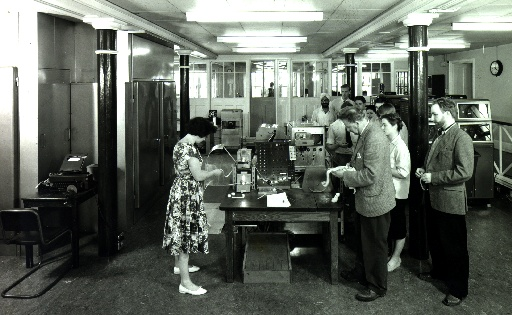
\includegraphics[width=1\textwidth]{imgs/EDSAC_2_1960.jpg}}
\end{frame}
\begin{frame}{Using HPC: Job Submission}
\begin{itemize}
\item{Compute resources are managed by a scheduler:\hfill\\\qquad\alert{SLURM}/PBS/SGE/LSF/\ldots}
\item{Jobs are submitted to the scheduler\hfill\\\qquad --- analogous to submitting jobs to a print queue\hfill\\\qquad --- a file (\emph{submission script}) is copied and queued\hfill\\\qquad \hphantom{---} for processing.}
\end{itemize}
\end{frame}

\begin{frame}{Using HPC: Job Submission}
\begin{itemize}
\item{Jobs are submitted from the \alert{login node}\hfill\\\qquad  --- not itself managed by the scheduler.}
\item{Jobs may be either non-interactive (\alert{batch}) or \alert{interactive}.}
\pause
\item{\alert{Batch} jobs run a shell script on the first of a list of allocated nodes.}
\item{\alert{Interactive} jobs provide a command line on the first of a list of allocated nodes.}
\end{itemize}
\end{frame}

\begin{frame}{Using HPC: Job Submission}
\begin{itemize}
\item{Jobs may use \alert{part} or \alert{all} of one or more nodes\hfill\\
\qquad --- the owner can specify \mbox{\tt --exclusive} to force exclusive\hfill\\\qquad\hphantom{---} node access.}
\item{Template submission scripts are available under\hfill\\
\qquad \alert{/usr/local/Cluster-Docs/SLURM}.}
\end{itemize}
\end{frame}

\begin{frame}[fragile]{Job Submission: Using SLURM}
\begin{itemize}
\item{Prepare a shell script and submit it to SLURM:}
\begin{semiverbatim}
\scriptsize
[abc123@login-a-1]\$ sbatch slurm_submission_script
Submitted batch job {\color{red}790299}
\end{semiverbatim}
\end{itemize}
\end{frame}

\begin{frame}[fragile]{Job Submission: Show Queue}
\begin{itemize}
\item{Submitted job scripts are copied and stored in a queue:}
\begin{semiverbatim}
\tiny
[abc123@login-a-1]\$ squeue -u abc123
             JOBID PARTITION     NAME     USER ST       TIME  NODES NODELIST(REASON)
            {\color{red}790299}   skylake     Test3  abc123 PD       0:00      2 (\only<1>{{\color{blue}Priority}}\only<2>{{\color{green}Resources}}\only<3>{{\color{red}AssocGrpCPUMinsLimit}})
            790290   skylake     Test2  abc123  R   27:56:10      2 cpu-a-[1,10]
\end{semiverbatim}
\end{itemize}
\end{frame}

\begin{frame}[fragile]{Job Submission: Monitor Job}
\begin{itemize}
\item{Examine a particular job:}
\begin{semiverbatim}
\scriptsize
[abc123@login-a-1]\$ scontrol show job={\color{red}790290}
\end{semiverbatim}
\end{itemize}
\end{frame}

\begin{frame}[fragile]{Job Submission: Cancel Job}
\begin{itemize}
\item{Cancel a particular job:}
\begin{semiverbatim}
\scriptsize
[abc123@login-a-1]\$ scancel {\color{red}790290}
\end{semiverbatim}
\end{itemize}
\end{frame}

\begin{frame}[fragile]{Job Submission: Scripts}
\begin{itemize}
\item{SLURM\hfill\\
In \alert{your home}, you will see template scripts for the different node types: \alert{slurm\_submit.peta4-skylake}, \alert{slurm\_submit.wilkes2}.}
  
\begin{semiverbatim}
\tiny
#!/bin/bash
#! Name of the job:
{\color<2->{red}#SBATCH} -J myjob
#! Which project should be charged:
{\color<2->{red}#SBATCH} -A TRAINING-CPU
#! How many whole nodes should be allocated?
{\color<2->{red}#SBATCH} --nodes=1
#! How many tasks will there be in total? (<= nodes*32)
{\color<2->{red}#SBATCH} --ntasks={\color<3->[rgb]{1,0,0}\only<1-3>{1}\only<4->{16}}
#! How much wallclock time will be required?
{\color<2->{red}#SBATCH} --time=02:00:00
#! Select partition:
{\color<2->{red}#SBATCH} -p skylake
...
\end{semiverbatim}
\item<2->{{\color{red}\#SBATCH} lines are \emph{structured comments}\hfill\\
\qquad --- correspond to sbatch command line options.}
\item<3->{\alert{The above job will be given {\color<3->[rgb]{1,0,0}\only<1-3>{1 cpu}\only<4->{16 cpus}} on 1 node for 2 hours (by default there is 1 task per node, and 1 cpu per task).}}
\end{itemize}
\end{frame}

\begin{frame}[fragile]{Job Submission: Accounting Commands}
\begin{itemize}
\item{How many core hours available do I have?}
\begin{semiverbatim}
\tiny
mybalance

User           Usage |        Account     Usage | Account Limit Available (hours)
---------- --------- + -------------- --------- + ------------- ---------
sjr20              3 |    SUPPORT-CPU     2,929 |    22,425,600 {\color{red}22,422,671}
sjr20              0 |    SUPPORT-GPU         0 |        87,600    {\color{red}87,600}
\end{semiverbatim}
\smallskip
\item{How many core hours does some other project or user have?}
\begin{semiverbatim}
\tiny
gbalance -p SUPPORT-CPU

User           Usage |        Account     Usage | Account Limit Available (hours)
---------- --------- + -------------- --------- + ------------- ---------

pfb29          2,925 |    SUPPORT-CPU     2,929 |    22,425,600 22,422,671
sjr20 *            3 |    SUPPORT-CPU     2,929 |    22,425,600 22,422,671
...
(Use -u for user.)
\end{semiverbatim}
\smallskip
\item{List all jobs charged to a project/user between certain times:}
\begin{semiverbatim}
\Tiny
gstatement -p SKYLAKE  -u xyz10 -s "2018-04-01-00:00:00" -e "2018-04-30-00:00:00" 
       JobID      User    Account    JobName  Partition                 End ExitCode      State  CompHrs 
------------ --------- ---------- ---------- ---------- ------------------- -------- ---------- -------- 
263              xyz10 support-c+ _interact+    skylake 2018-04-18T19:44:40      0:0    TIMEOUT      1.0
264              xyz10 support-c+ _interact+    skylake 2018-04-18T19:48:07      0:0 CANCELLED+      0.1
275              xyz10 support-c+ _interact+    skylake             Unknown      0:0    RUNNING      0.3
...
\end{semiverbatim}
\end{itemize}
\end{frame}

\subsection{Single Node Jobs}
\begin{frame}[fragile]{Job Submission: Single Node Jobs}
\begin{itemize}
\item{Serial jobs requiring large memory, or OpenMP codes.}
\begin{semiverbatim}
\scriptsize
#!/bin/bash
\ldots
#SBATCH --nodes=1
\uncover<2-|handout:2->{{\color{red}#SBATCH --ntasks=1
# Default is 1 task per node}} 
\uncover<3-|handout:2->{{\color{red}#SBATCH --cpus-per-task=\only<3-5|handout:2>{1}\only<6,8-|handout:3,5->{32 # Whole node}\only<7|handout:4>{16  # Half node}
\only<3-5|handout:2>{# Default is 1 cpu (core) per task}}}
\uncover<4-5|handout:2>{{\color{red}#SBATCH --mem=5990
# Memory per node in MB - default is pro rata by cpu number}}
\uncover<5|handout:2>{{\color{red}# Increasing --mem or --cpus-per-task implicitly increases the other}}
\ldots
\uncover<6-|handout:3->{{\color{red}export OMP\_NUM\_THREADS=\only<6|handout:3>{32}\only<7-|handout:4->{16}  # For OpenMP across \only<6|handout:3>{32}\only<7-|handout:4->{16} cores\only<8-|handout:5->{ (using all memory)}}}
\$application \$options
\ldots
\end{semiverbatim}
\end{itemize}
\end{frame}

\subsection{MPI Jobs}
\begin{frame}[fragile]{Job Submission: MPI Jobs}
\begin{itemize}
\item{Parallel job across multiple nodes.}
\begin{semiverbatim}
\scriptsize
#!/bin/bash
\ldots
#SBATCH --nodes={\color{red}4}
#SBATCH --ntasks=\alert{\only<1|handout:1>{128}\only<2-|handout:2->{64}}     # \only<1|handout:1>{i.e.\ {\color[rgb]{0,0.8,0}32}}\only<2-|handout:2->{i.e.\ {\color[rgb]{0,0.8,0} 16}}x{\color{red}4} MPI tasks in total.
\uncover<2-|handout:2->{{\color{red}#SBATCH --cpus-per-task=2}}
\ldots
mpirun\only<2-|handout:2->{ -ppn {\color[rgb]{0,0.8,0}16}} -np \alert{\only<1|handout:1>{128}\only<2-|handout:2->{64}} \$application \$options
\ldots
\end{semiverbatim}
\item<3-|handout:2->{\small SLURM-aware MPI launches remote tasks via SLURM.}
\item<3-|handout:2->{\small The template script uses \$SLURM\_TASKS\_PER\_NODE to set PPN.}
\end{itemize}
\end{frame}

\subsection{Hybrid Jobs}
\begin{frame}[fragile]{Job Submission: Hybrid Jobs}
\begin{itemize}
\item{Parallel jobs using both MPI and OpenMP.}
\begin{semiverbatim}
\scriptsize
#!/bin/bash
\ldots
#SBATCH --nodes={\color{red}4}
#SBATCH --ntasks=\alert{64}     # i.e.\ {\color[rgb]{0,0.8,0}16}x{\color{red}4} MPI tasks in total.
#SBATCH --cpus-per-task={\color{brown}2}
\ldots
{\color{brown}export OMP\_NUM\_THREADS=2   # i.e.\ 2 threads per MPI task.}
mpirun -ppn {\color[rgb]{0,0.8,0}16} -np \alert{64} \$application \$options
\ldots
\end{semiverbatim}
\item<2->{\small This job uses \alert{128 CPUs} (each MPI task splits into 2 OpenMP threads).}
\end{itemize}
\end{frame}

\subsection{High Throughput Jobs}
\begin{frame}[fragile]{Job Submission: High Throughput Jobs}
\begin{itemize}
\item{Multiple serial jobs across multiple nodes.}
\item{Use \alert{srun} to launch tasks (\alert{job steps}) within a job.}
\begin{semiverbatim}
\scriptsize
#!/bin/bash
\ldots
#SBATCH --nodes=2
\ldots
cd directory\_for\_job1
\alert{srun} {\color<3>{red}--exclusive} {\color<2>{red}-N 1 -n 1} \$application \$options\_for\_job1 > output 2> err {\color<4>{red}&}
cd directory\_for\_job2
\alert{srun} {\color<3>{red}--exclusive} {\color<2>{red}-N 1 -n 1} \$application \$options\_for\_job2 > output 2> err {\color<4>{red}&}
...
cd directory\_for\_job64
\alert{srun} {\color<3>{red}--exclusive} {\color<2>{red}-N 1 -n 1} \$application \$options\_for\_job64 > output 2> err {\color<4>{red}&}
{\color<5>{red}wait}
\end{semiverbatim}
\end{itemize}
\end{frame}

\section{HPC Job Submission}

\subsection{README}
\begin{frame}{README: Job Scripts!}
If you are attending the HPC Course:
\begin{itemize} 
\item{Use job\textunderscore script for the exerises when running the exercises during the course}
\item {Use slurm\textunderscore submit.peta4-skylake if running the exercises outside of the course}
\item {I recommend you make a copy of the job script for each exercise}
\end{itemize}
\end{frame}

\subsection{Exercise 11: High Throughput Jobs}
\begin{frame}{Exercise 11: Submitting a Matlab job}
\begin{itemize}
\item{Submit a job which will run \alert{matlab} on the \alert{file.m} command file (which contains just the \alert{ver} command).}
\visible<2->{\begin{description}
\item[\emph{Hints:}]{\scriptsize\begin{enumerate}
\item{Edit the \alert{job\_script} in your exercises directory.}
\item{In the module load section: \alert{module load matlab/r2017b{}}}
\item{Set the value of application to\hfill\break{}\alert{\"{}matlab -nodesktop -nosplash -nojvm\"{}}}
\item{Set the value of options to \alert{\"{}-r file\"{}}}
\item{Submit the job with \alert{sbatch job\_script}. The jobid is then printed.}
\item{Watch the job in the queue with \alert{squeue}.}
\item{After it has disappeared, open the output file \alert{slurm-jobid.out} in your editor. It should contain a list of licensed Matlab features.}
  \item{For more demanding work you can increase the available memory by increasing the number of cpus.}
  \end{enumerate}%
}
\end{description}}
\end{itemize}
\end{frame}

\subsection{Exercise 12: High Throughput Jobs}
\begin{frame}{Exercise 12: Submitting compiled code}
\begin{itemize}
\item{Submit a job which will run a copy of your hello program on 1 cpu.}
\visible<2->{\begin{description}
\item[\emph{Hints:}]{\scriptsize\begin{enumerate}
\item{Edit the script \alert{job\_script} in your exercises directory. Set:\hfill\\
\alert{\#SBATCH --nodes=1}\hfill\\
\alert{\#SBATCH --ntasks=1}\hfill\\
\alert{application="./hello"}}
\item{Submit the job with \alert{sbatch job\_script}. The jobid is then printed.}
\item{Watch the job in the queue with \alert{squeue}.}
\item{After it has disappeared, open the output file \alert{slurm-jobid.out} in your editor. There should be exactly one ``Hello, World!'' message.}
\end{enumerate}%
}
\end{description}}
\end{itemize}
\end{frame}

\subsection{Interactive Jobs}
\begin{frame}[fragile]{Job Submission: Interactive}
\begin{itemize}
\item{Compute nodes are accessible via SSH \alert{while you have a job running on them}.}
\pause
\item{Alternatively, submit an interactive job:}
\begin{semiverbatim}
\alert{sintr -A TRAINING-CPU -N1 -n8 -t 2:0:0}
\end{semiverbatim}
\medskip
\pause
\item{Within the window (screen session):}
\begin{itemize}
\item[$\ast$]{Launches a shell on the first node (when the job starts).}
\item[$\ast$]{Graphical applications should display correctly.}
\item[$\ast$]{Create new shells with \alert{ctrl-a c}, navigate with \alert{ctrl-a n} and \alert{ctrl-a p}.}
\item[$\ast$]{\alert{ssh} or \alert{srun} can be used to start processes on any nodes in the job.}
\item[$\ast$]{SLURM-aware MPI will do this automatically.}
\end{itemize}
\end{itemize}
\end{frame}

\section{Array Jobs}
\subsection{Array Jobs}
\begin{frame}[fragile]{Job Submission: Array Jobs}
\begin{itemize}
\item{\alert{$http://slurm.schedmd.com/job\_array.html$}}
\item{Used for submitting and managing large sets of similar jobs.}
\item{Each job in the array has the same \alert{initial} options.}
\item{SLURM}
\begin{semiverbatim}
\scriptsize
[abc123@login-a-1]\$ sbatch --array=\only<1,2>{{\color{red}1-7}}\only<2>{{\color{red}:2}}\only<3->{{\color{red}1,3,5,7}} -A TRAINING-CPU submit\_script
Submitted batch job {\color[rgb]{0,0.6,0}791609}
\tiny
\uncover<4->{[abc123@login-a-1]\$ squeue -u abc123
             JOBID PARTITION     NAME     USER ST       TIME  NODES NODELIST(REASON)
          {\color[rgb]{0,0.6,0}791609}\_{\color{red}1} skylake      hpl    abc123  R       0:06      1 cpu-a-6
          {\color[rgb]{0,0.6,0}791609}\_{\color{red}3} skylake      hpl    abc123  R       0:06      1 cpu-a-16
          {\color[rgb]{0,0.6,0}791609}\_{\color{red}5} skylake      hpl    abc123  R       0:06      1 cpu-a-7
          {\color[rgb]{0,0.6,0}791609}\_{\color{red}7} skylake      hpl    abc123  R       0:06      1 cpu-a-7
}
\end{semiverbatim}
\uncover<5->{\centerline{{\color[rgb]{0,0.6,0}791609}\_{\color{red}1}, {\color[rgb]{0,0.6,0}791609}\_{\color{red}3}, {\color[rgb]{0,0.6,0}791609}\_{\color{red}5}, {\color[rgb]{0,0.6,0}791609}\_{\color{red}7}}}
\smallskip
\uncover<6->{\centerline{i.e.\ \$\{{\color[rgb]{0,0.6,0}SLURM\_ARRAY\_JOB\_ID}\}\_\$\{{\color{red}SLURM\_ARRAY\_TASK\_ID}\}}}
\smallskip
\uncover<7->{\leftline{\small SLURM\_ARRAY\_JOB\_ID${}={}$SLURM\_JOBID for the first element.}}
\end{itemize}
\end{frame}

\begin{frame}[fragile]{Job Submission: Array Jobs (ctd)}
\begin{itemize}
\item{Updates can be applied to specific array elements using \$\{{\color[rgb]{0,0.6,0}SLURM\_ARRAY\_JOB\_ID}\}\_\$\{{\color{red}SLURM\_ARRAY\_TASK\_ID}\}}
\item{Alternatively operate on the entire array via \$\{{\color[rgb]{0,0.6,0}SLURM\_ARRAY\_JOB\_ID}\}}.
\item{Some commands still require the SLURM\_JOB\_ID (sacct, sreport, sshare, sstat and a few others).}
\pause
\item{Exercise 7 - Array Jobs.}
\end{itemize}
\end{frame}

\subsection{Excercise 13: Array Jobs}
\begin{frame}{Exercise 13: Array Jobs}
\begin{itemize}
\item{Submit your last job in the form of an array with indices 1-32. Use -H with sbatch to mark the array as held (so that it won't run immediately).}
\visible<2->{\begin{description}
\item[\emph{Hints:}]{\scriptsize\begin{enumerate}
\item{Use \alert{sbatch -H -{}-array=1-32 job\_script}}
\item{Use \alert{squeue -u userid} to see your array job. Note that \alert{-r} reports each array element individually.}
\end{enumerate}%
}
\end{description}}
\item{Release array element 1 and allow it to run. Then release the others.}
\visible<3->{\begin{description}
\item[\emph{Hints:}]{\scriptsize\begin{enumerate}
\item{Use \alert{scontrol release \$\{{SLURM\_ARRAY\_JOB\_ID}\}\_{{\color{red}1}}}}
\item{Use \alert{squeue -u userid} again to watch what happens.}
\item{Release the others with\hfill\break
\null\qquad scontrol release \$\{{SLURM\_ARRAY\_JOB\_ID}\}\hfill\break
i.e. use the array id to release the entire array.}
  \item{When all the jobs complete you should have 32 slurm-\$\{SLURM\_ARRAY\_JOB\_ID\}\_N.out files saying hello from various cpus on possibly multiple nodes.}
\end{enumerate}%
}
\end{description}}
\end{itemize}
\end{frame}

\subsection{Scheduling}
\begin{frame}{Scheduling}
\begin{itemize}
\item{SLURM scheduling is multifactor:}
  \pause
\begin{itemize}
\item{\alert{QoS} --- payer or non-payer?}
  \pause
\item{\alert{Age} --- how long has the job waited?\hfill\\\qquad
  \alert{Don't cancel jobs that seem to wait too long.}}
  \pause
\item{\alert{Fair Share} --- how much recent usage?\hfill\\\qquad
  \alert{Payers with little recent usage receive boost (not implemented yet).}}
  \pause
\item{\alert{sprio -j jobid}}
\end{itemize}
\pause
\item{\alert{Backfilling}}
\begin{itemize}
  \item{Promote lower priority jobs into gaps left by higher priority jobs.}
    \item{Demands that the higher priority jobs not be delayed.}
    \item{Relies on reasonably accurate wall time requests for this to work.}
      \item{Jobs of default length will not backfill readily.}
\end{itemize}
\end{itemize}
\end{frame}

\subsection{Wait Times}
\begin{frame}{Wait Times}
  \begin{itemize}
 \item{12 or 36 hour job walltimes are permitted.}
    \pause
    \item {SL3 jobs, 12hrs (non payers), SL2 and 1, 36hrs (payers)}
  \item{\alert{This sets the timescale at busy times (\emph{without} backfilling).}}
    \pause
  \item{Use backfilling when possible.}
  \item{Short (1 hour or less) jobs have higher throughput.}
\end{itemize}
\end{frame}

\subsection{Checkpointing}
\begin{frame}{Checkpointing}
  \begin{itemize}
  \item{Insurance against failures during long jobs.}
  \item{Restart from checkpoints to work around finite job length.}
    \pause
  \item{Application native methods are best. Failing that $\ldots$}
  \end{itemize}
\end{frame}

\subsection{Scheduling Top Tips}
\begin{frame}{Job Submission: Scheduling Top Dos \& Don'ts}
\begin{itemize}
\item{\textbf{Do \ldots}}
\begin{itemize}
\item{Give reasonably accurate wall times (allows \alert{backfilling}).}
\item{Check your balance occasionally (\alert{mybalance}).}
\item{Test on a small scale first.}
\item{Implement \alert{checkpointing} if possible (reduces resource wastage).}
\end{itemize}
\medskip
\item{\textbf{Don't \ldots}}
\begin{itemize}
\item{Request more than you need\hfill\\
\qquad --- you will wait longer and use more credits.}
\item{Cancel jobs unnecessarily\hfill\\
\qquad ---  priority increases over time.}
\end{itemize}
\end{itemize}
\end{frame}

